% major update 8/4/11
% typo fixes 12/5/11
% --------------------------------------------------------------------------
%\documentclass[onecolumn,11pt]{ieeetran}
\documentclass[]{siamltex}
\usepackage{graphics,stfloats,amssymb,amsmath,amsfonts,epsfig}
\usepackage{algorithm}
\usepackage{algorithmic}
\usepackage{hyperref}
\usepackage{verbatim}
%\usepackage[named]{algo}

% Example definitions
% -------------------
\def\x{{\mathbf x}}
\def\L{{\cal L}}
\def\half{\frac{1}{2}}
\def\alphamax{\alpha_{\mbox{\tiny max}}}
\def\alphamin{\alpha_{\mbox{\tiny min}}}


% more useful abbreviations
% -------------------------
\newcommand{\R}{\mathbb{R}}
\newcommand{\C}{\mathbb{C}}
\newcommand{\btheta}{\mbox{\boldmath $\theta$}}
\newcommand{\bgamma}{\mbox{\boldmath $\gamma$}}
\newcommand{\bbeta}{\mbox{\boldmath  $\beta$}}
\newcommand{\balpha}{\mbox{\boldmath $\alpha$}}
\newcommand{\bDelta}{\mbox{\boldmath $\Delta$}}
\newcommand{\bdelta}{\mbox{\boldmath $\delta$}}
\newcommand{\bPsi}{\mbox{\boldmath   $\Psi$}}
\newcommand{\bphi}{\mbox{\boldmath   $\phi$}}
\newcommand{\bpi}{\mbox{\boldmath    $\pi$}}
\newcommand{\btau}{\mbox{\boldmath   $\tau$}}
\newcommand{\blambda}{\mbox{\boldmath $\lambda$}}
\newcommand{\bTheta}{\mbox{\boldmath $\Theta$}}
\newcommand{\bone}{\mbox{\boldmath   $1$}}
\newcommand{\Loewner}[0]{\preceq}
\newcommand{\Hessmat}{{\cal H}}
\newcommand{\Bmat}{{\bf B}}
\newcommand{\Amat}{{\bf A}}
\newcommand{\bx}{{\bf x}}
\newcommand{\gradv}{{\bf g}}
\newcommand{\cG}{{\cal G}}
\newcommand{\cS}{{\cal S}}
\newcommand{\cT}{{\cal T}}
\newcommand{\trace}{\mbox{\rm trace}}
\newcommand{\tv}{\tilde{v}}
\newcommand{\gammaC}{\gamma_C}

\def\noprint#1{}
\def\swcomment#1{{\em [SW: #1]}}
\def\dmcomment#1{{\em [DM: #1]}}
\def\swresolved#1{}
\def\dmresolved#1{}
\def\sparsa{SpaRSA\ }
\def\bi{\begin{itemize}}
\def\ei{\end{itemize}}
\def\beq{\begin{equation}}
\def\eeq{\end{equation}}
\def\eqnok#1{(\ref{#1})}

% theorem environments
% \newtheorem{theorem}{Theorem}
% \newtheorem{lemma}[theorem]{Lemma}
% \newtheorem{corollary}[theorem]{Corollary}

% baselinestretch definition is important!!
% \renewcommand{\baselinestretch}{1.565}

% \ninept

% Title.
% ------
\title{EECS 451 Fall 2013 EXAM 2 \hspace{1.2cm} NOVEMBER 19}

\begin{document}
%\ninept
%
\maketitle
This exam is closed-book. You are allowed two notes pages, $8.5 \times 11$, front and back. You must be able to read the page without any technology (e.g. magnifying devices). You are also given the DTFT, DFS, and DFT tables from the book at the end of these exam papers.

\vspace{4mm} \textbf{Please justify your answers; No credit will be given without justification.} Write neatly and \fbox{put a box around your final answer,} unless the answer is a proof or unless otherwise specified. Notice the point values on each problem-- \textbf{the total is 90 points}. Most importantly: good luck!!

\vspace{1cm}
Print name: \makebox[3in]{\hrulefill} 

\vspace{4mm}
Grad or Undergrad (circle one)

\vspace{4mm}
HONOR CODE PLEDGE:
``I have neither given nor received aid on this exam, nor have I
concealed any violations of the honor code."

\vspace{4mm}
Sign the pledge: \makebox[3in]{\hrulefill} 
\vspace{1cm}

\newpage
\begin{enumerate}
\item (10 points, 5 points each sub-part.) The continuous-time signal $$x_c(t) = \sin(30 \pi t ) + \cos (180 \pi t)$$ is sampled with a sampling period $T$ to obtain the discrete-time signal $$x[n] = \sin\left(\frac{\pi n}{12}\right) + \cos\left(\frac{\pi n}{2}\right)\;.$$ 
% OSB 2nd edition 4.4

\vspace{5mm} 
\begin{enumerate}
\item Determine a choice for $T$ consistent with this information. 

\vspace{1cm} 
\textbf{Solution.} $T = \frac{1}{360}$.

\vspace{1cm}
\item Is your choice for $T$ in Part (a) unique? If so, explain why. If not, specify another choice of $T$ consistent with the information given.

\vspace{1cm} 
\textbf{Solution.} It's not unique because $$\sin\left(\frac{\pi n}{12}\right) = \sin \left(\frac{\pi n}{12} + 2\pi k n\right) = \sin \left( \left(\frac{1}{12} + 2 k\right) \pi n\right)  $$ for any integer $k$ and 
$$\cos\left(\frac{\pi n}{2}\right) = \cos\left(\frac{\pi n}{2} + 2\pi m n\right) = \cos\left( \left( \frac{1}{2} + 2m\right) \pi n \right)$$ for any integer $m$. Therefore we could find any other $T'$ that satisfies $$30 T' = \frac{1}{12} + 2k \quad \text{ and } 180 T' = \frac{1}{2} + 2m$$ simultaneously, where we get to pick $k$ and $m$ such that this is possible. We can do this for any $k$ and $m$ such that $$\frac{1}{360} + \frac{2k}{30} = \frac{1}{360}+\frac{2m}{180} \implies 6k=m\;.$$ So choosing $k=1$, $m=6$ we get $$T' = \frac{25}{360}\;.$$

\end{enumerate}


\newpage
\item (15 points total, see point values below) Consider the systems shown below. Suppose that $H_1(\omega)$ is fixed and known. 
% OSB 2nd edition 4.29, GATech PS 7 solutions

$$x_1[n] \rightarrow \fbox{$\uparrow 2$} \rightarrow v[n]  \rightarrow \fbox{$H_1(\omega)$}  \rightarrow q[n]\rightarrow \fbox{$\downarrow 2$} \rightarrow y_1[n]\;,$$

$$x_2[n] \rightarrow \fbox{$H_2(\omega)$} \rightarrow y_2[n]\;.$$

\vspace{3mm} Remember that \fbox{$\uparrow M$} means we insert $M-1$ zeros between samples and \fbox{$\downarrow M$} means we take every $M^{th}$ sample.

\vspace{3mm} 
\begin{enumerate}
\item (5 points) What is $V(\omega)$ in terms of $X_1(\omega)$? What is $Q(\omega)$ in terms of $X_1(\omega)$ and $H_1(\omega)$?

\vspace{1cm} 
\textbf{Solution.} $V(\omega) = X_1(2\omega)$. $Q(\omega) = V(\omega) H_1(\omega) = X_1(2\omega) H_1(\omega)$.

\vspace{1cm} \item (10 points) Find $H_2(\omega)$, the frequency response of an LTI system, such that $y_1[n] = y_2[n]$ when $x_1[n] = x_2[n]$ (in other words, the outputs are the same when the inputs are the same).

\vspace{1cm} 
\textbf{Solution.} $Y_1(\omega) = \frac{1}{2} \left( Q\left(\frac{\omega}{2}\right) + Q\left(\frac{\omega}{2} + \pi\right) \right)$. So that means we have 
\begin{align*}
Y_1(\omega) &= \frac{1}{2} \left[ X_1\left(2\frac{\omega}{2}\right)  H_1\left(\frac{\omega}{2}\right)   +  X_1\left(2\left(\frac{\omega}{2}+\pi\right)\right)  H_1\left(\frac{\omega}{2} + \pi\right)  \right] \\
&= \frac{1}{2} \left[ X_1(\omega)  H_1\left(\frac{\omega}{2}\right)   +  X_1(\omega + 2\pi)  H_1\left(\frac{\omega}{2} + \pi\right)  \right] \\
&= \frac{1}{2} \left(  H_1\left(\frac{\omega}{2}\right)   +  H_1\left(\frac{\omega}{2} + \pi\right)  \right) X_1(\omega) 
\end{align*} because $X_1(\omega + 2\pi)  = X_1(\omega)$. Therefore, we should take $$H_2(\omega) = \frac{1}{2} \left(  H_1\left(\frac{\omega}{2}\right)   +  H_1\left(\frac{\omega}{2} + \pi\right) \right)\;.$$

\end{enumerate}




\newpage

\item (30 points total, plus 5 points extra credit, see point values below.) 
% OSB 4.38 2nd edition, Solution in SP05_PS7_soln of GA Tech
\begin{enumerate}
\item (12 points) Consider the following system. $$x_c(t)  \rightarrow \fbox{C/D with period $T$}  \rightarrow x[n] \rightarrow \fbox{$\uparrow L$}  \rightarrow v[n] \rightarrow \fbox{$H(\omega)$} \rightarrow q[n] $$

The filter $H(\omega)$ is defined as $$H(\omega) = \left\{ \begin{matrix} 1, & |\omega| < \pi/L \\ 0 , & \pi/L < |\omega| < \pi\end{matrix} \right. \;.$$

$X_c(\Omega)$ is given in this figure. What do $V(\omega)$ and $Q(\omega)$ look like? Draw them on a plot with clear labels of the axes, the locations where the signal touches the x-axis, and the height of the signal.

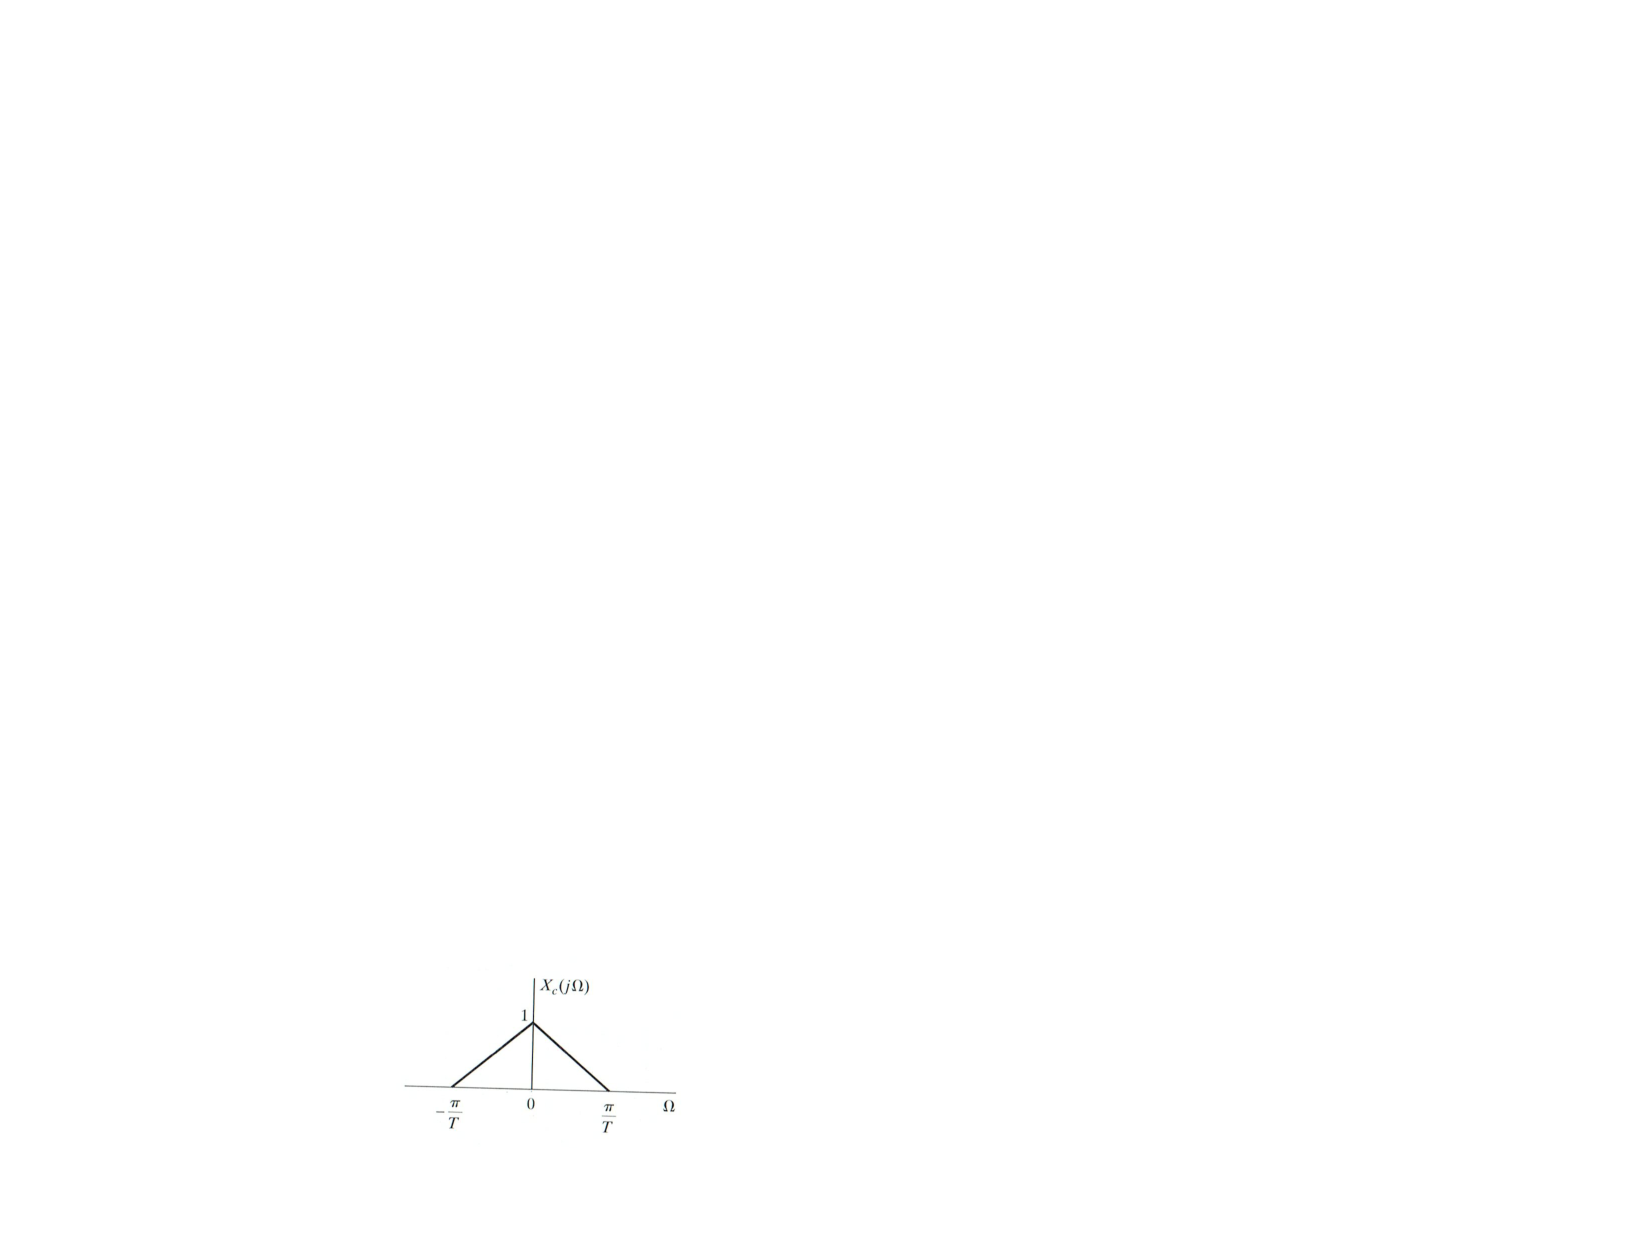
\includegraphics{osb4382}

\newpage
\item (18 points) Now continue the system from part (a) as follows, where $q[n]$ is the output of the system in part (a).

$$q[n] \rightarrow \fbox{Modulator} \rightarrow y[n] \rightarrow  \fbox{D/C with period $T' = T/L$} \rightarrow y_c(t)$$


The box labeled ``Modulator'' takes the input sequence $w[n]$ and multiplies it by $(-1)^n$: $$y[n] = (-1)^n q[n]\;.$$ Draw $Y(\omega)$, the DTFT of $y[n]$, and $Y_c(\Omega)$, the CTFT of $y_c(t)$. Again be sure to clearly label the axes, locations where the signal touches the x-axis, and the height of the signal.

\vspace{4in}
\item (5 points, extra credit) Can we swap the modulator with our LTI filter $H(\omega)$ and still get the same overall system? Why or why not?
\end{enumerate}

\newpage
\item (20 points total, see point values below.) The given sequence $x_1[n]$ is periodic with period $N=5$. We would like to convolve it with the $h[n]$ given. 
\vspace{4mm}

 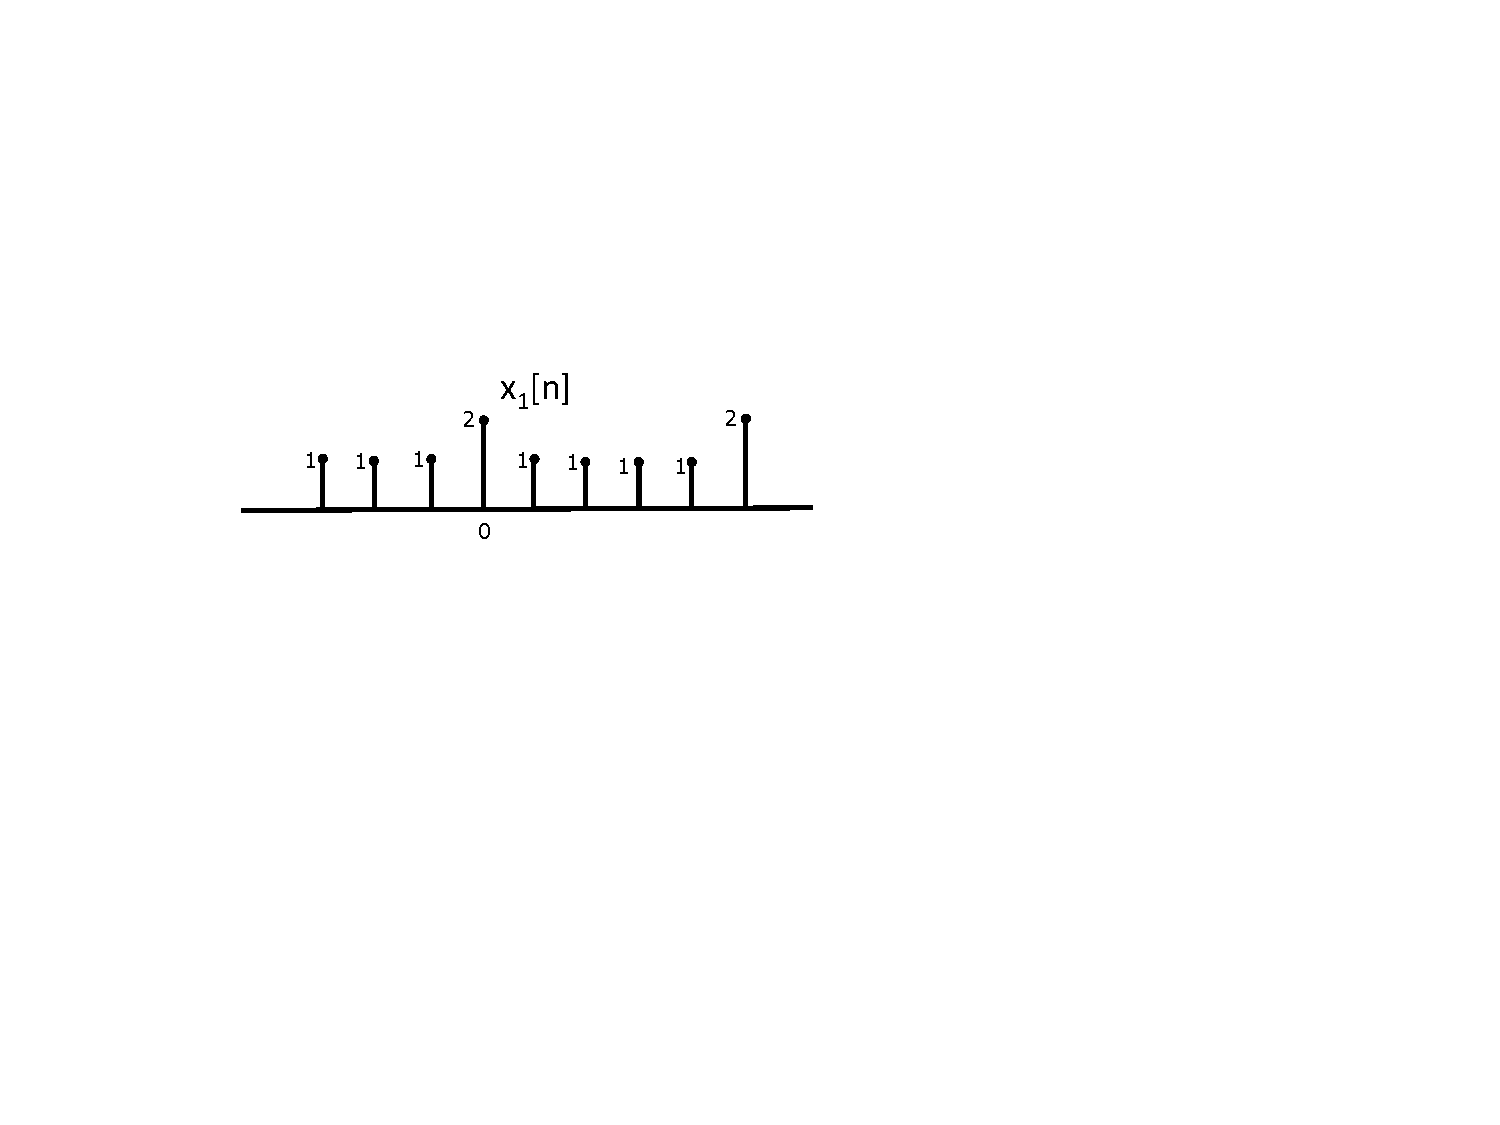
\includegraphics[width=0.43\textwidth]{x1}  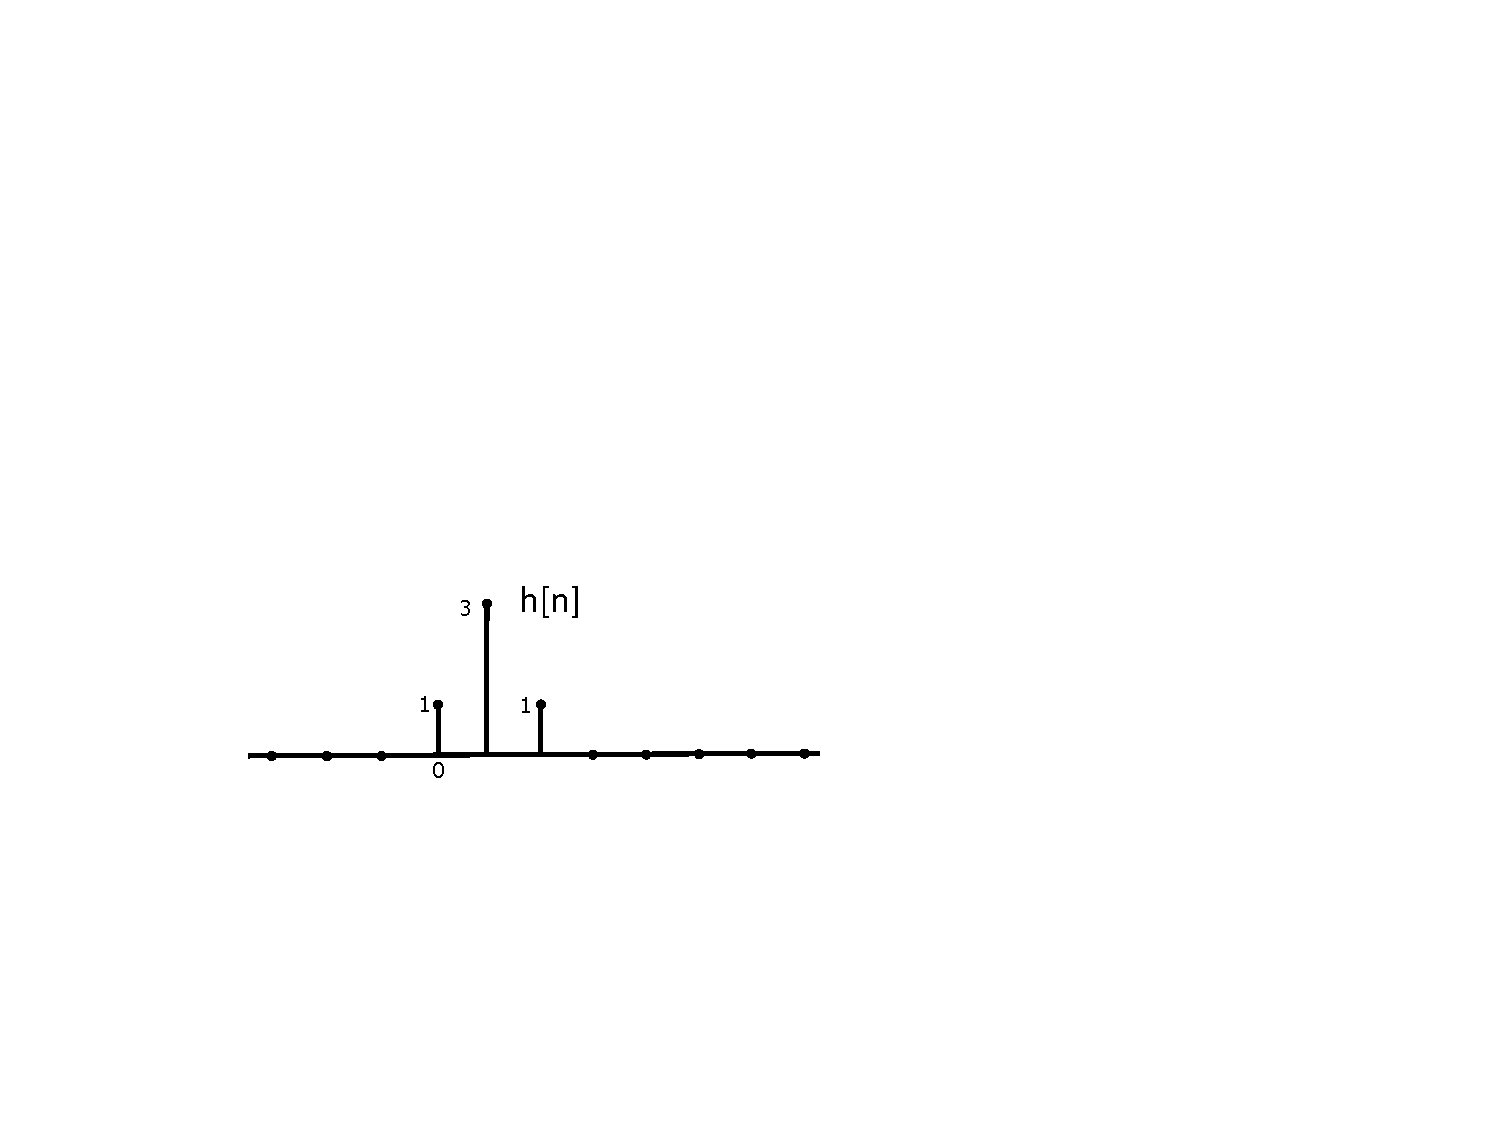
\includegraphics[width=0.43\textwidth]{h}


\begin{enumerate} 
\item (5 points) What is the result of the length-$N=5$ periodic convolution between these two sequences?

\vspace{3in}
\item (5 points) Now consider $x_2[n]$, which is zero for all indices not shown. What is the result of the length-$N=5$ circular convolution of $x_2[n]$ and $h[n]$?

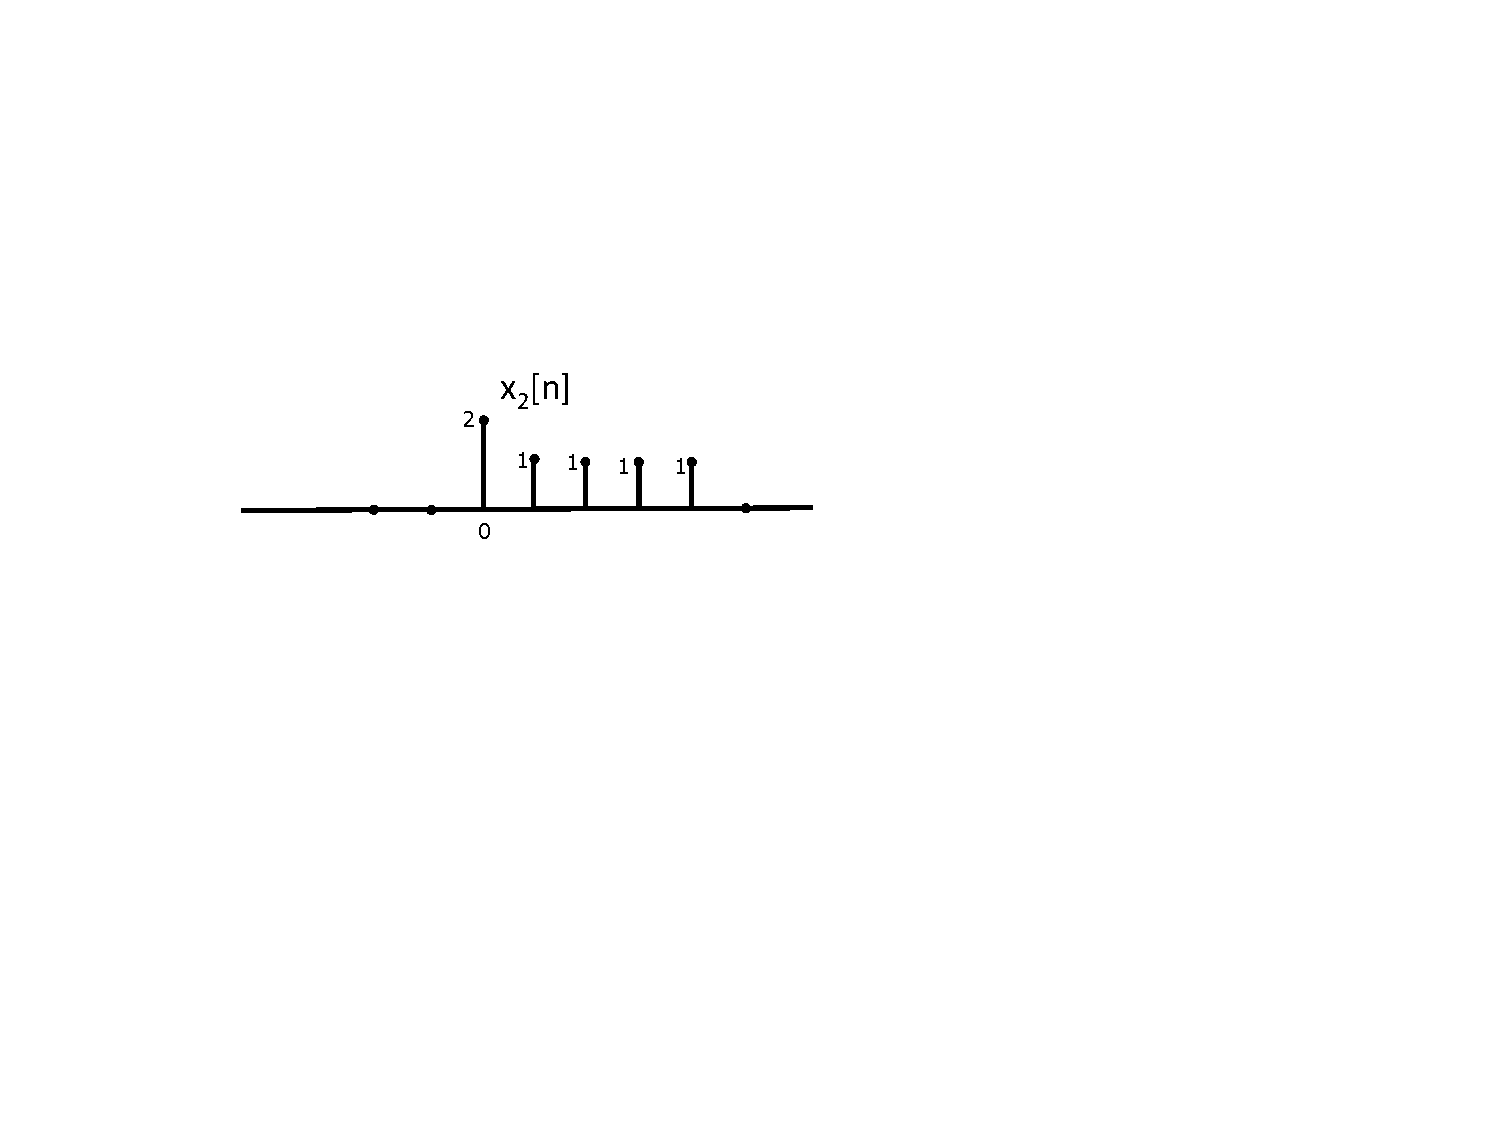
\includegraphics[width=0.45\textwidth]{x2}

\newpage
\item (10 points) Now consider that we would like to implement the following LTI system, where $H(\omega)$ is the DTFT of $h[n]$ given above.

$$x_2[n]  \rightarrow \fbox{$H(\omega)$} \rightarrow y_2[n]\;.$$

Instead we need to implement it on a computer, so we'll use the DFT as follows.

$$x_2[n] \rightarrow  \fbox{M-point DFT}  \rightarrow \fbox{$G[k]$}\rightarrow  \fbox{M-point IDFT}  \rightarrow y_2[n]\;.$$

\begin{enumerate} 
\item Describe what we must do to $x_2[n]$ and/or $h[n]$ to guarantee that $$y_2[n] = x_2[n]*h[n],$$ 

i.e. the output is the linear convolution of $x_2[n]$ and  $h[n]$.

\vspace{1in} 
\item What is the minimum value $M$ can be to guarantee we get the linear convolution?

\vspace{.5in}
\item Suppose we took $M=10$. In this case, describe how $G[k]$ relates to $H[k]$, the $N=5$-point DFT of $h[n]$.
\end{enumerate}
\end{enumerate}

\newpage
\item (15 points) For the FFT, we learned how to break a length-8 DFT into two DFTs of length-4. Use the same approach to show how you could break a length-12 DFT into three DFTs of length-4. 











\end{enumerate}


\end{document}
